\section{Evaluations}
\begin{itemize}
    \item We built a NanoPU prototype on top of the open source RISC-V Rocket Core. Cite chipyard XXX.
    \item For the prototype we focused on building the NanoPU NIC datapath, NIC-Core interface, and a minimal operating system (the NanoKernel).
    \item Our prototype does not implement a full NanoPU:
    \begin{itemize}
        \item It does not make any modifications to the memory hierarchy.
        \item It does not implement any encryption or decryption.
        \item The NIC and the core run at the same clock rate, hence the CDC FIFOs are not included.
        \item The prototype assumes all messages consist of a single packet. It does not implement a reliable transport protocol.
    \end{itemize}
    \item We will assume a 3 GHz clock for our RISC-V prototype in order to report performance numbers, because this is a typical clock speed for a CPU. \steve{Should we report performance numbers in terms of clock cycles or Gbps and nanoseconds?}
    \item Probably need to include a description of how well we believe IceNIC represents a modern state-of-the-art NIC.
\end{itemize}

\subsection{Microbenchmarks}
This section describes a set of microbenchmarks that characterize various aspects of the NanoPU architecture.

\paragraph{Timing Analysis.} We synthesized both our NanoPU RISC-V prototype as well as a standard RISC-V core with a traditional NIC (IceNIC) to a modern FPGA (Xilinx Ultrascale+) in order to analyze the critical paths in each design.
We found that the critical path in both designs is in the L2 cache, and hence our NanoPU prototype is able to achieve the same clock rate as a traditional RISC-V system.

\paragraph{Basic Latency/Throughput Performance Analysis.} The latency of the NanoPU's TX path is 11 cycles for a single word message, which is measured from the cycle when an application writes the word to when the word is placed on the network (not including the MAC processing).
The corresponding latency of the RX path is 6 cycles.
Figure~\ref{fig:loopback-latency} shows the loopback latency for various packet lengths for both our NanoPU prototype and the traditional DMA-based IceNIC.

Table\ref{tab:throughput} shows the TX and RX throughput for 64B packets for both our NanoPU prototype and IceNIC. 

\begin{table}[]
\begin{center}
\begin{tabular}{|c|c|c|c|c|}
\hline
                & \textbf{RX bytes/cycle} & \textbf{RX Gbps} & \textbf{TX bytes/cycle} & \textbf{TX Gbps} \\ \hline
\textbf{NanoPU} & 3.01                    & 72               & 7.65                    & 185              \\ \hline
\textbf{IceNIC} & 0.58                    & 14               & 1.16                    & 28               \\ \hline
\end{tabular}
\caption{TX and RX throughput achievable by both our NanoPU prototype and IceNIC.}
\label{tab:throughput}
\end{center}
\end{table}

\begin{itemize}
    \item TX/RX throughput for 64B packets
\end{itemize}

\begin{figure}
  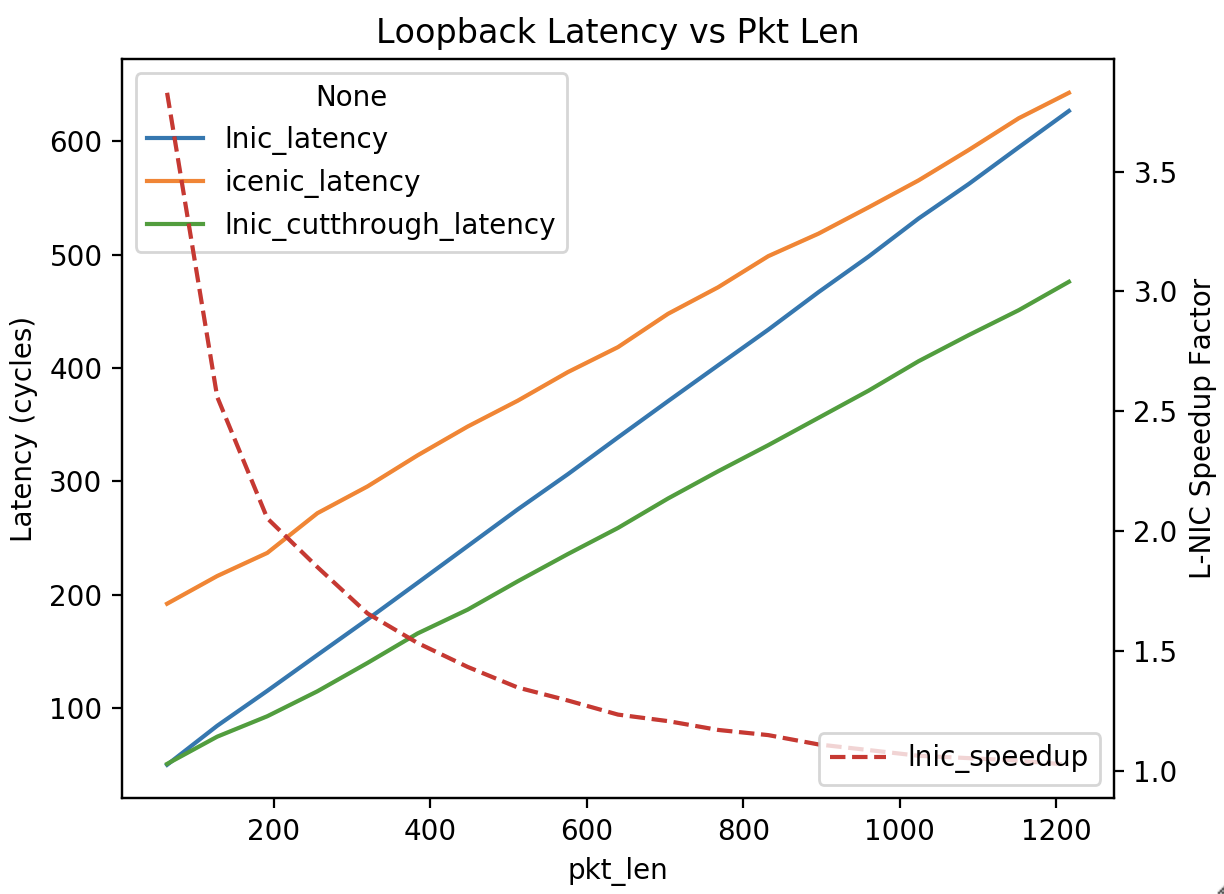
\includegraphics[width=\linewidth]{./figures/loopback-latency}
  \caption{NanoPU vs Traditional net-core-net loopback latency for various packet sizes.}
  \label{fig:loopback-latency}
\end{figure}

\paragraph{Basic NanoKernel Performance Analaysis.}
\begin{itemize}
    \item NanoKernel context switch latency
\end{itemize}

\subsection{Bare Metal Application Evaluations}
\begin{itemize}
    \item This section shows the reduction in average latency as a result of the hardware fast path to the core of the CPU.
    \item Streaming application (NFV style)
    \item Neural Network inference node
    \item Othello
    \item N-body simulation
\end{itemize}

\begin{figure}
  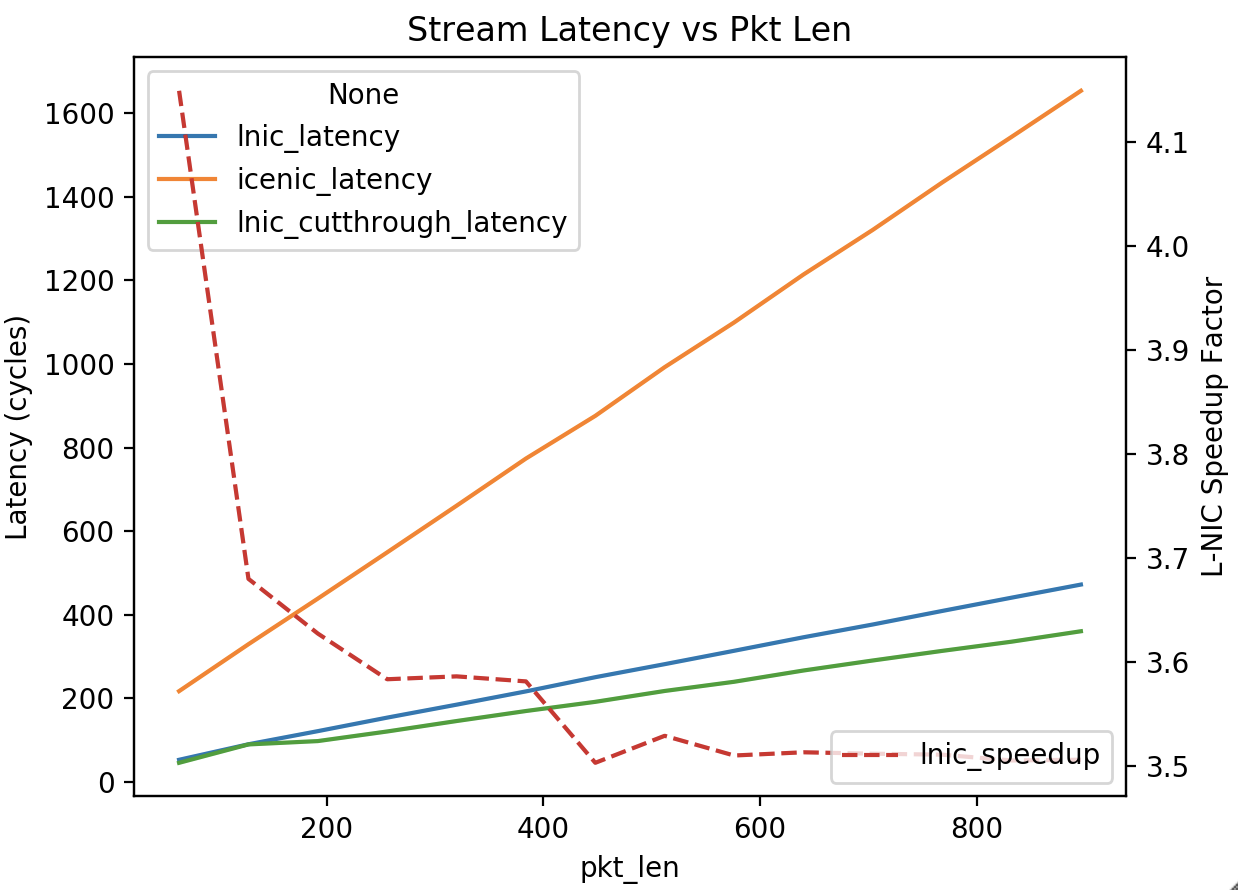
\includegraphics[width=\linewidth]{./figures/stream-latency}
  \caption{NanoPU vs Traditional NFV-style streaming application latency for various packet sizes.}
  \label{fig:stream_latency}
\end{figure}

\begin{figure}
  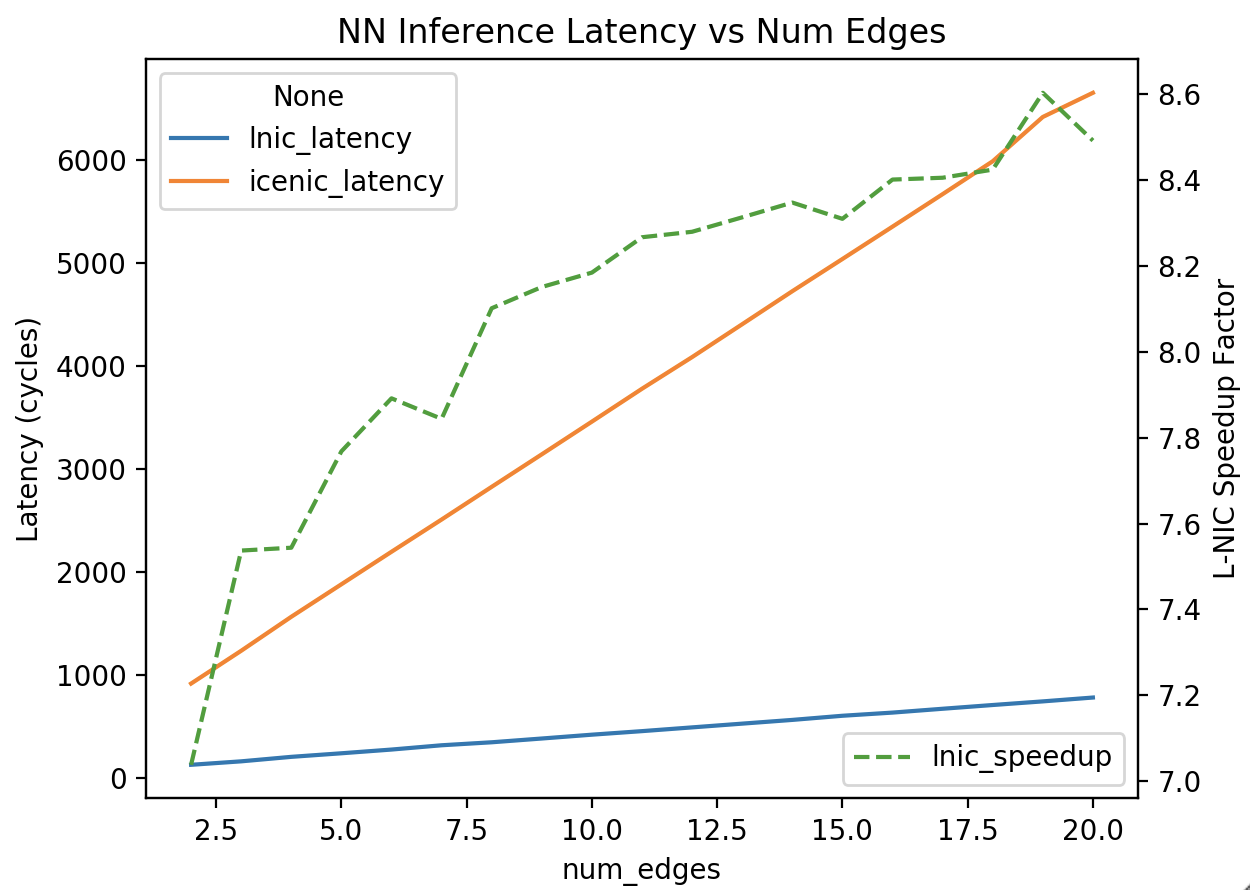
\includegraphics[width=\linewidth]{./figures/nn-inference-latency}
  \caption{NanoPU vs Traditional neural network node latency for various number of incoming edges.}
  \label{fig:nn_latency}
\end{figure}

\begin{figure}
  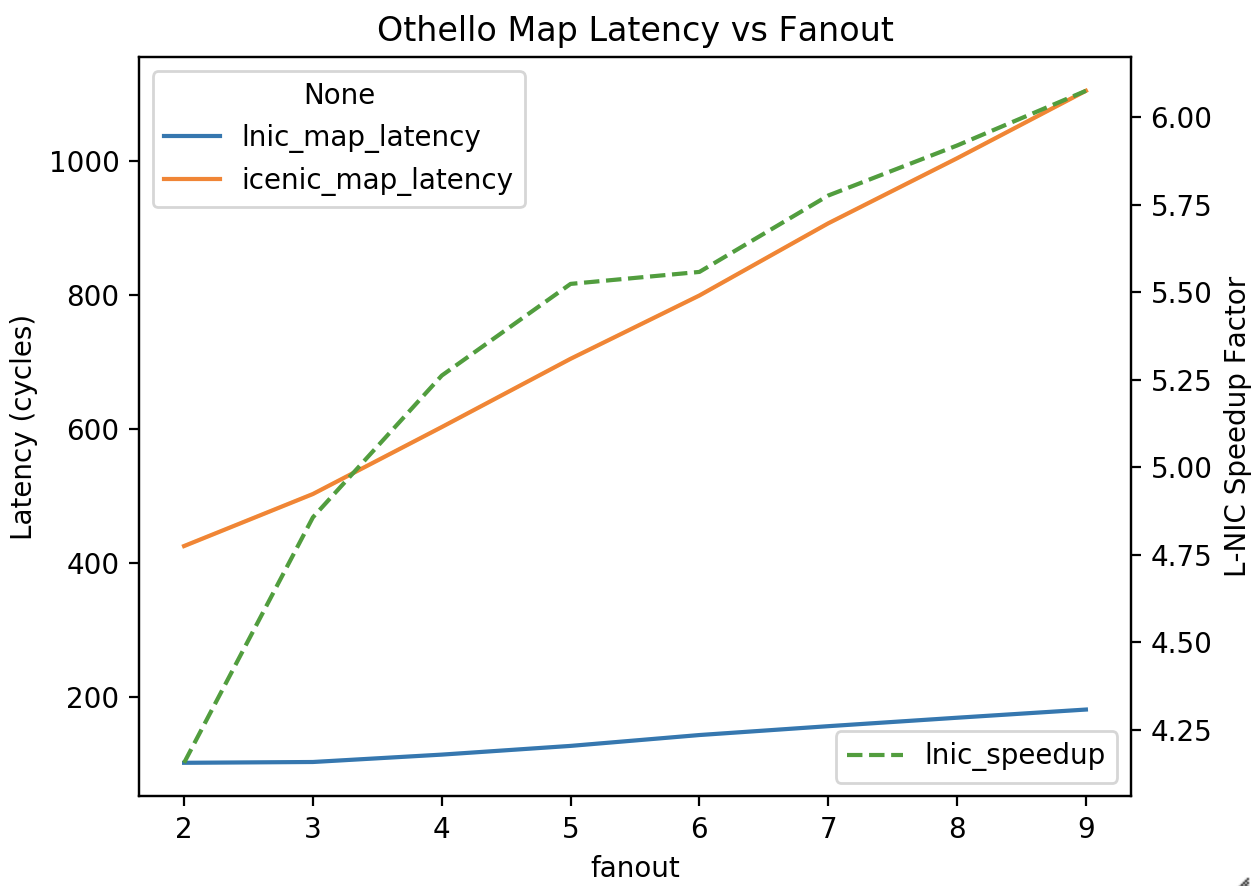
\includegraphics[width=\linewidth]{./figures/othello-map-latency}
  \caption{NanoPU vs Traditional Othello map latency for various degrees of fanout.}
  \label{fig:othello_map_latency}
\end{figure}

\begin{figure}
  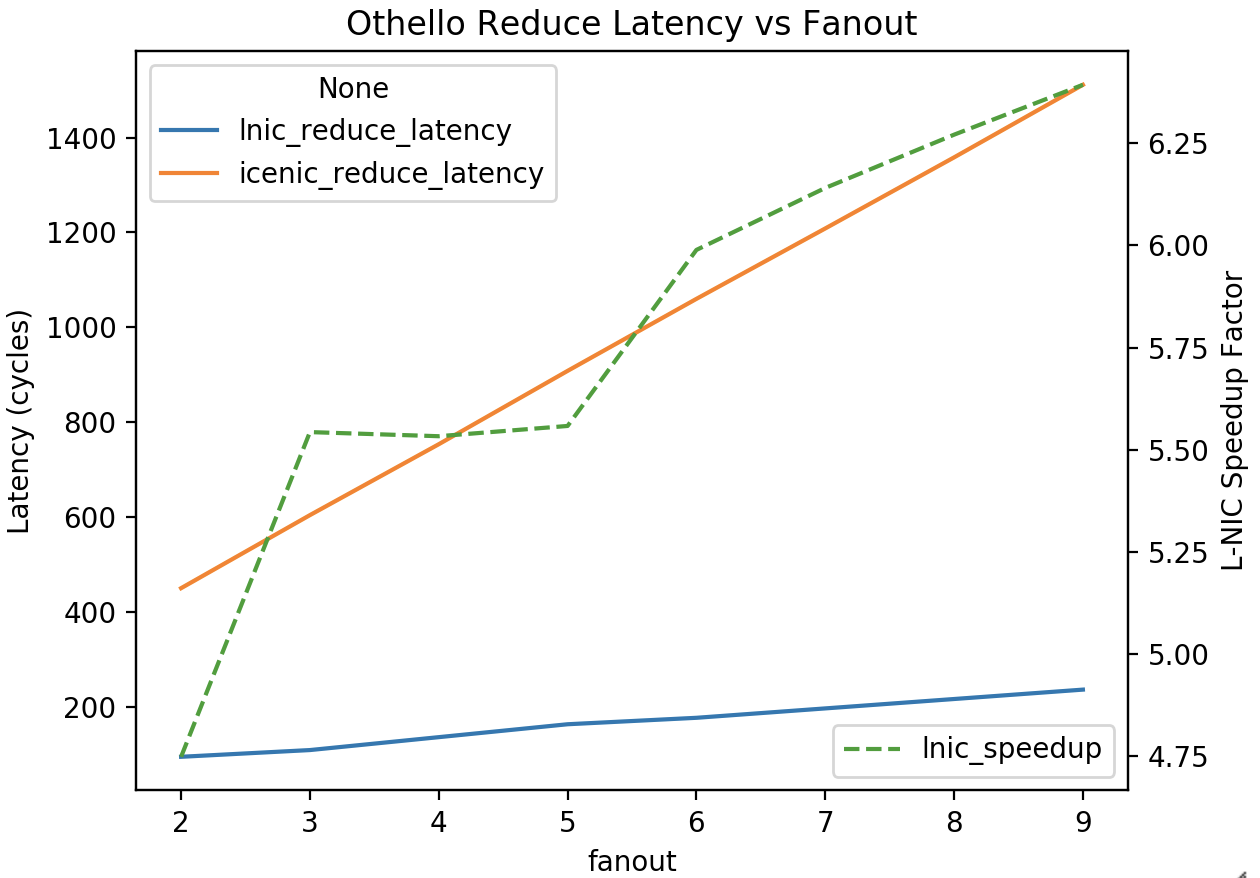
\includegraphics[width=\linewidth]{./figures/othello-reduce-latency}
  \caption{NanoPU vs Traditional Othello reduce latency for various degrees of fanout.}
  \label{fig:othello_reduce_latency}
\end{figure}

\subsection{Thread Scheduling Evaluations}
\begin{itemize}
    \item This section shows the reduction in tail latency as a result of NIC-driven thread scheduling for nanoservice applications.
    \item Compare Linux-style timer interrupt driven scheduling to NIC driven thread scheduling on the NanoPU.
    \item Explain the experiment set up.
    \item Show that NIC driven scheduling has much lower tail latency.
\end{itemize}

\subsection{Large Scale Nanoservice Evaluation}
\begin{itemize}
    \item Show evaluations of large scale (1000's of NanoPU cores) nanoservice deployment being used to implement an N-body simulation.
    \item Maybe compare to ChanGa.
    \item Show that the nanoservices implementation can perform the simulation much faster.
\end{itemize}
